\begin{figure}[htbp]
\centering
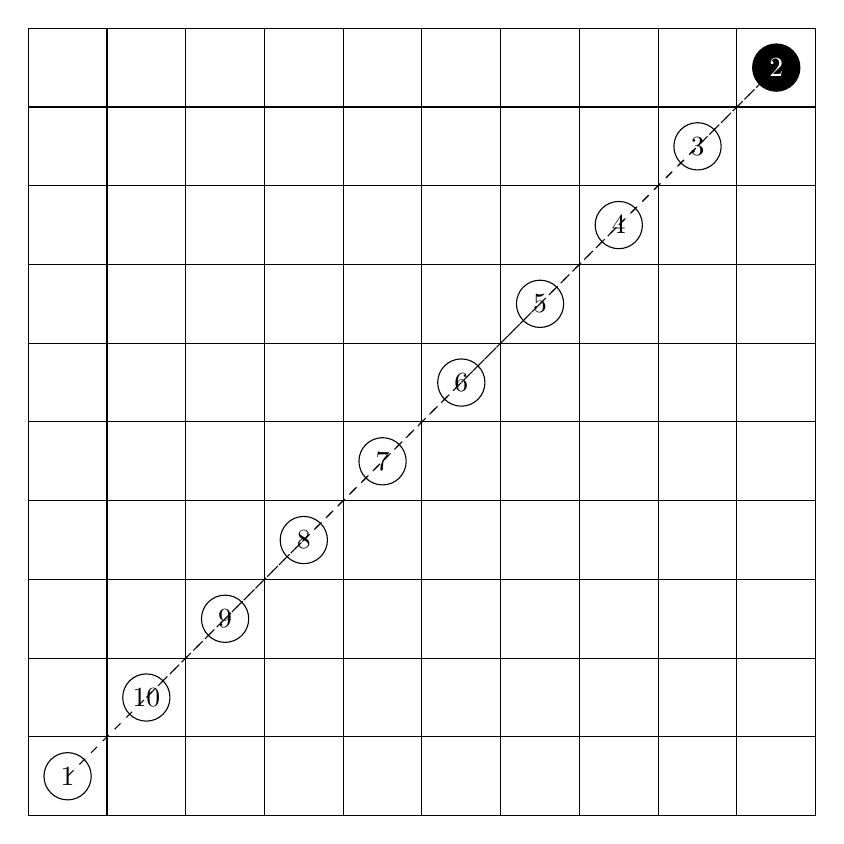
\begin{tikzpicture}

	\draw[xshift=0.5cm, yshift=0.5cm] (0,0) grid (10,10);
	\draw (1, 1) circle [radius=0.3];
	\draw (2, 2) circle [radius=0.3];
	\draw (3, 3) circle [radius=0.3];
	\draw (4, 4)  circle [radius=0.3];
	\draw (5, 5)  circle [radius=0.3];
	\draw (6, 6) circle [radius=0.3];
	\draw (7, 7)  circle [radius=0.3];
	\draw (8, 8)  circle [radius=0.3];
	\draw (9, 9)  circle [radius=0.3];
	\draw[fill=black] (10, 10)  circle [radius=0.3];

	\draw (1, 1) node {1};
	\draw (2, 2) node {10};
	\draw (3, 3) node{9};
	\draw (4, 4) node{8};
	\draw (5, 5) node{7};
	\draw (6, 6) node{6};
	\draw (7, 7) node{5};
	\draw (8, 8) node{4};
	\draw (9, 9) node{3};
	\draw[white] (10, 10) node{2};
	
	\draw[style=dashed] (1,1) -- (10,10);
	\draw[style=dashed] (2,2) -- (3,3);
	\draw[style=dashed] (3,3) -- (4,4);
	\draw[style=dashed] (4,4) -- (5,5);
	\draw[style=dashed] (5,5) -- (6,6);
	\draw[style=dashed] (6,6) -- (7,7);
	\draw[style=dashed] (7,7) -- (8,8);
	\draw[style=dashed] (8,8) -- (9,9);
	\draw[style=dashed] (9,9) -- (10,10);
\end{tikzpicture}

\caption{Soluci\'on del caso de peor entrada de la Figura \ref{ej_2:peor}}
\label{ej_2:peor:sol}
\end{figure}
